%%
%% Template chap2.tex
%%

\chapter{Experiment 1: Learning with Random Sampling}
\label{cha:expt1}



\section{Experimental Protocol}
\label{sec:protocol1}



\section{Results and Discussion}
\label{sec:results1}

\subsection{Colour Indices and Feature Selection}






\subsection{Comparison of Reddening Correction Sets}

\begin{figure}[tbp]
	\centering
	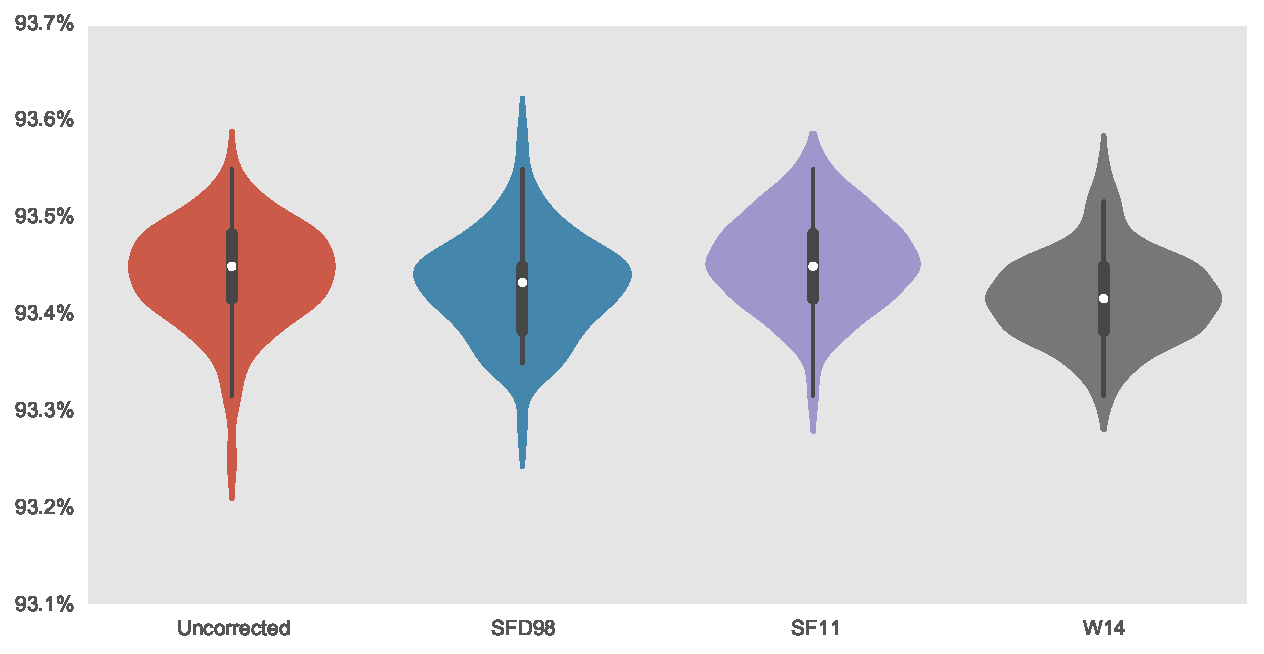
\includegraphics[width=\textwidth]{figures/violin_reddening_correction}
	\caption{Comparing the accuracy rates using 4 correction sets.}
	\label{fig:reddeningviolin}
\end{figure}

\subsection{Learning Curves with Random Sampling}

\begin{figure}[tbp]
	\centering
	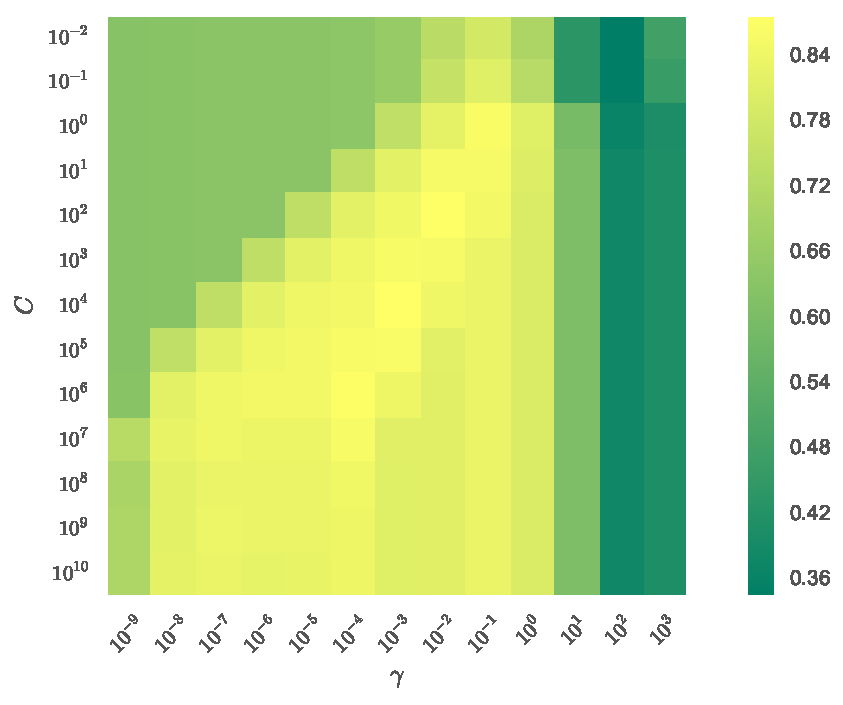
\includegraphics[width=0.7\textwidth]{figures/heat_gridsearch_svm_rbf}
	\caption{Accuracy rate heat map of the hyperparameters of SVM (RBF) for the SDSS.}
	\label{fig:sdss_heat_rbf}
\end{figure}

\begin{figure}[tbp]
	\centering
	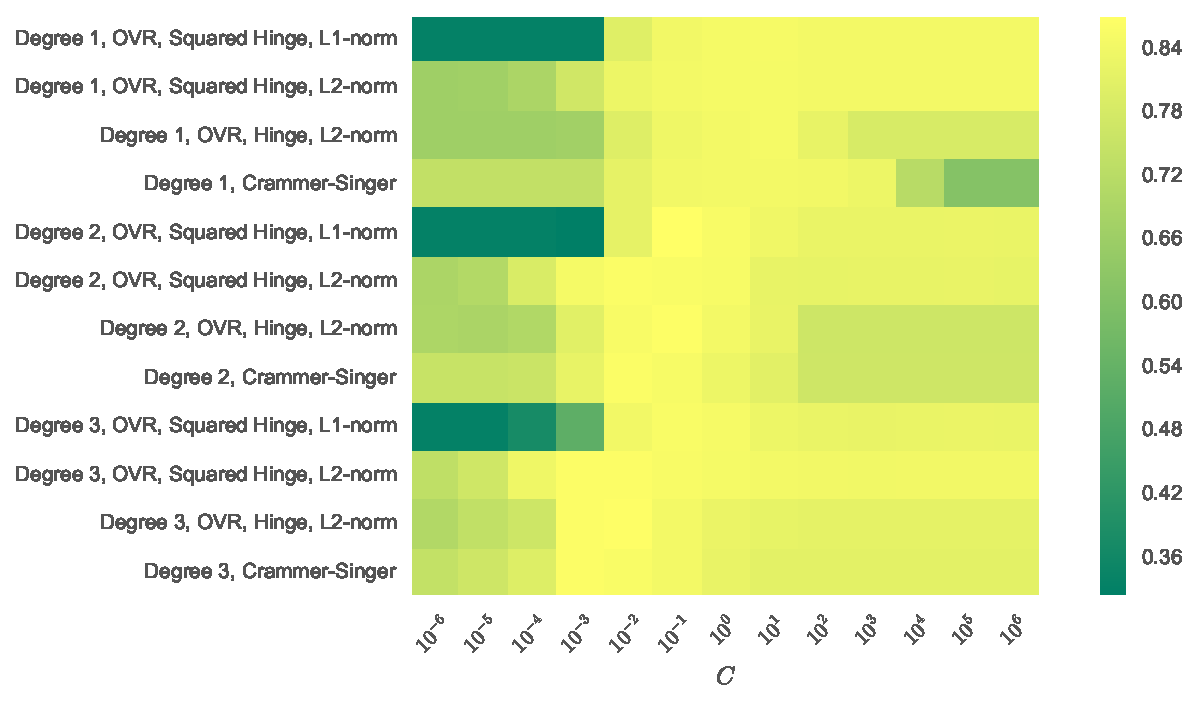
\includegraphics[width=\textwidth]{figures/heat_gridsearch_svm_poly}
	\caption{Accuracy rate heat map of the hyperparameters of SVM (Polynomial) for the SDSS.}
	\label{fig:sdss_heat_poly}
\end{figure}

\begin{figure}[tbp]
	\centering
	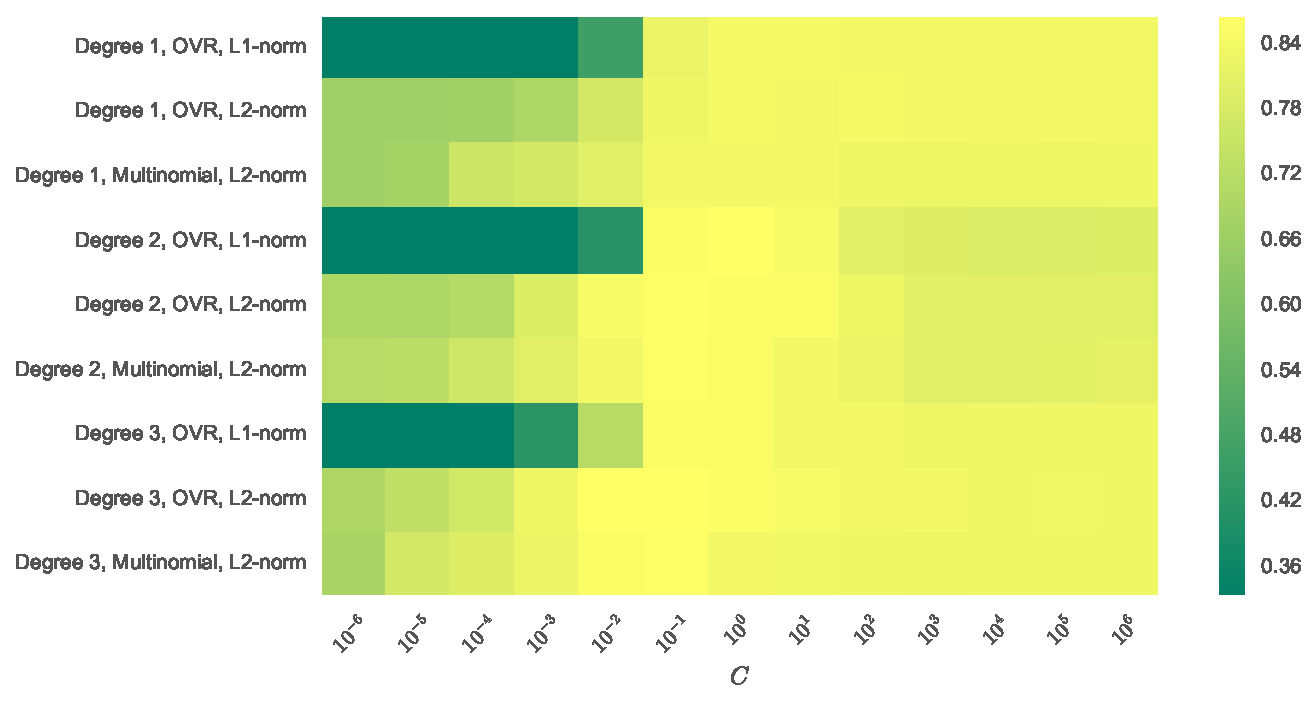
\includegraphics[width=\textwidth]{figures/heat_gridsearch_logistic}
	\caption{Accuracy rate heat map of the hyperparameters of Logistic Regression for the SDSS.}
	\label{fig:sdss_heat_logistic}
\end{figure}

\begin{figure}[tbp]
	\centering
	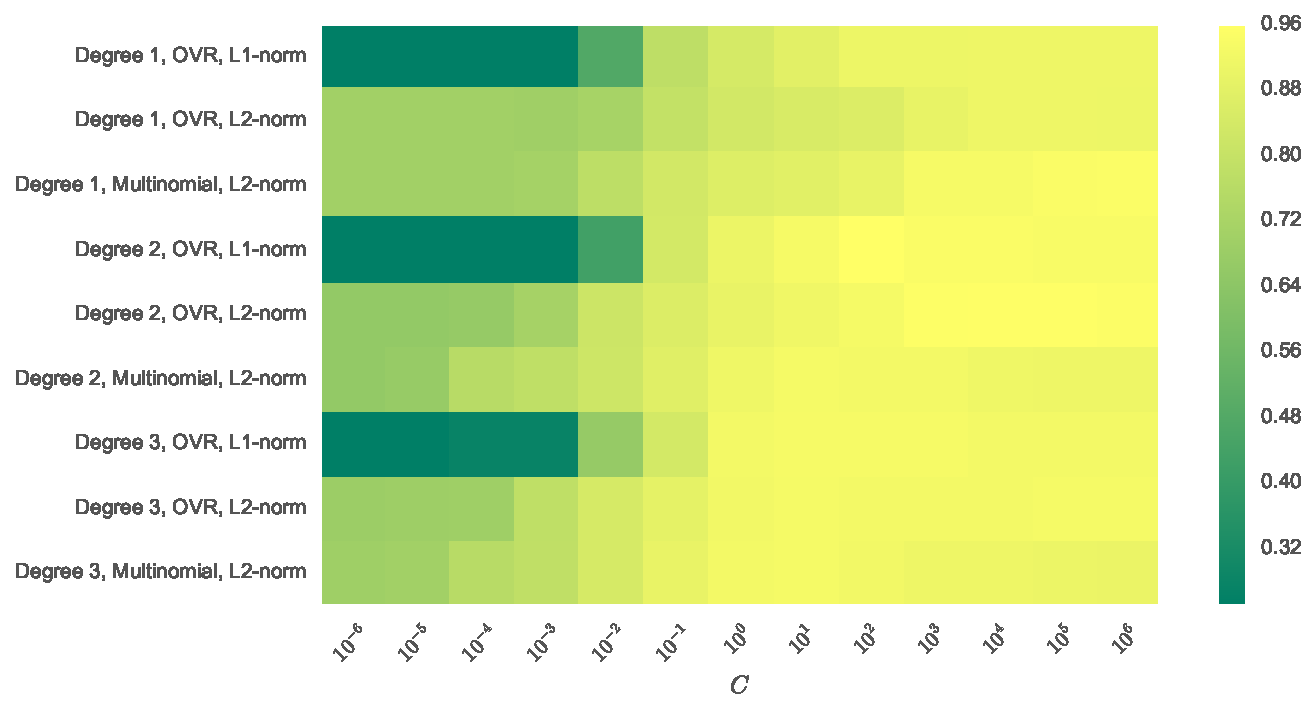
\includegraphics[width=\textwidth]{figures/heat_vstatlas_vgridsearch_logistic}
	\caption{Accuracy rate heat map of the hyperparameters of Logistic Regression for the VST ATLAS.}
	\label{fig:vst_heat_logistic}
\end{figure}


\begin{figure}[tbp]
	\centering
	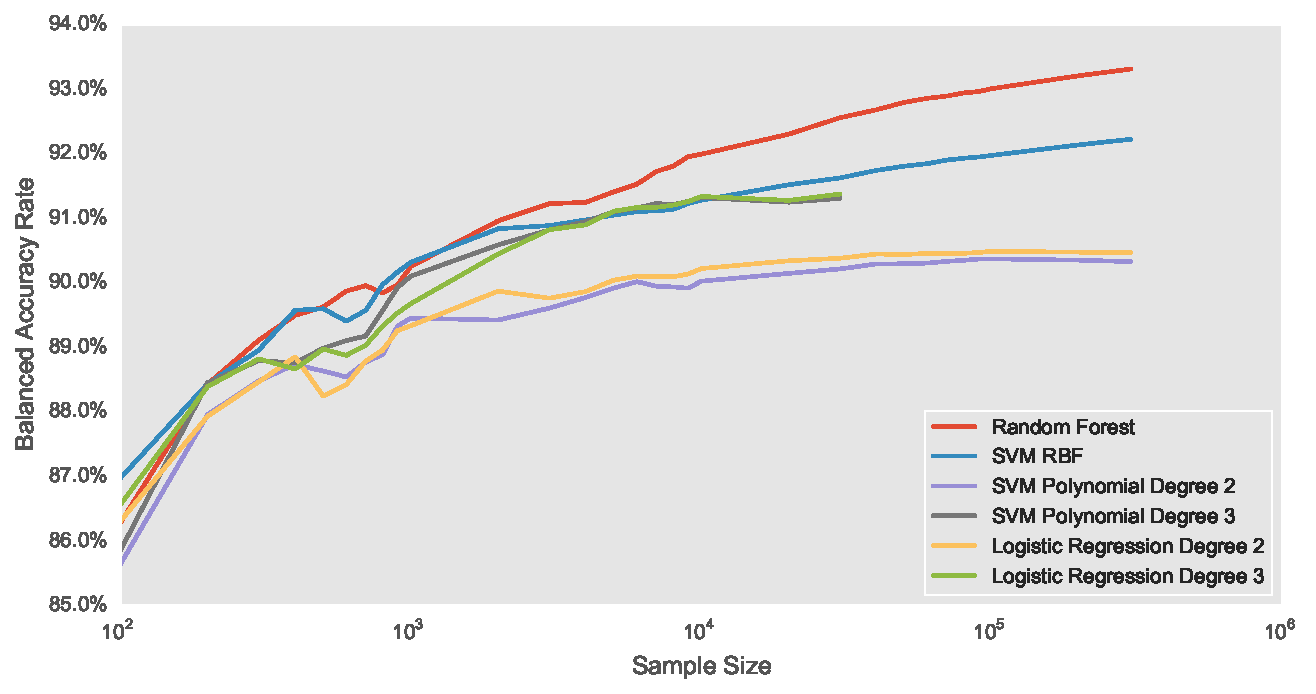
\includegraphics[width=\textwidth]{figures/learning_curves}
	\caption{SDSS learning curves with random sampling.}
	\label{fig:sdss_learning}
\end{figure}





\subsection{Class Proportion Estimation}

\begin{figure}[p]
	\centering
	\begin{subfigure}{\textwidth}
		\centering
		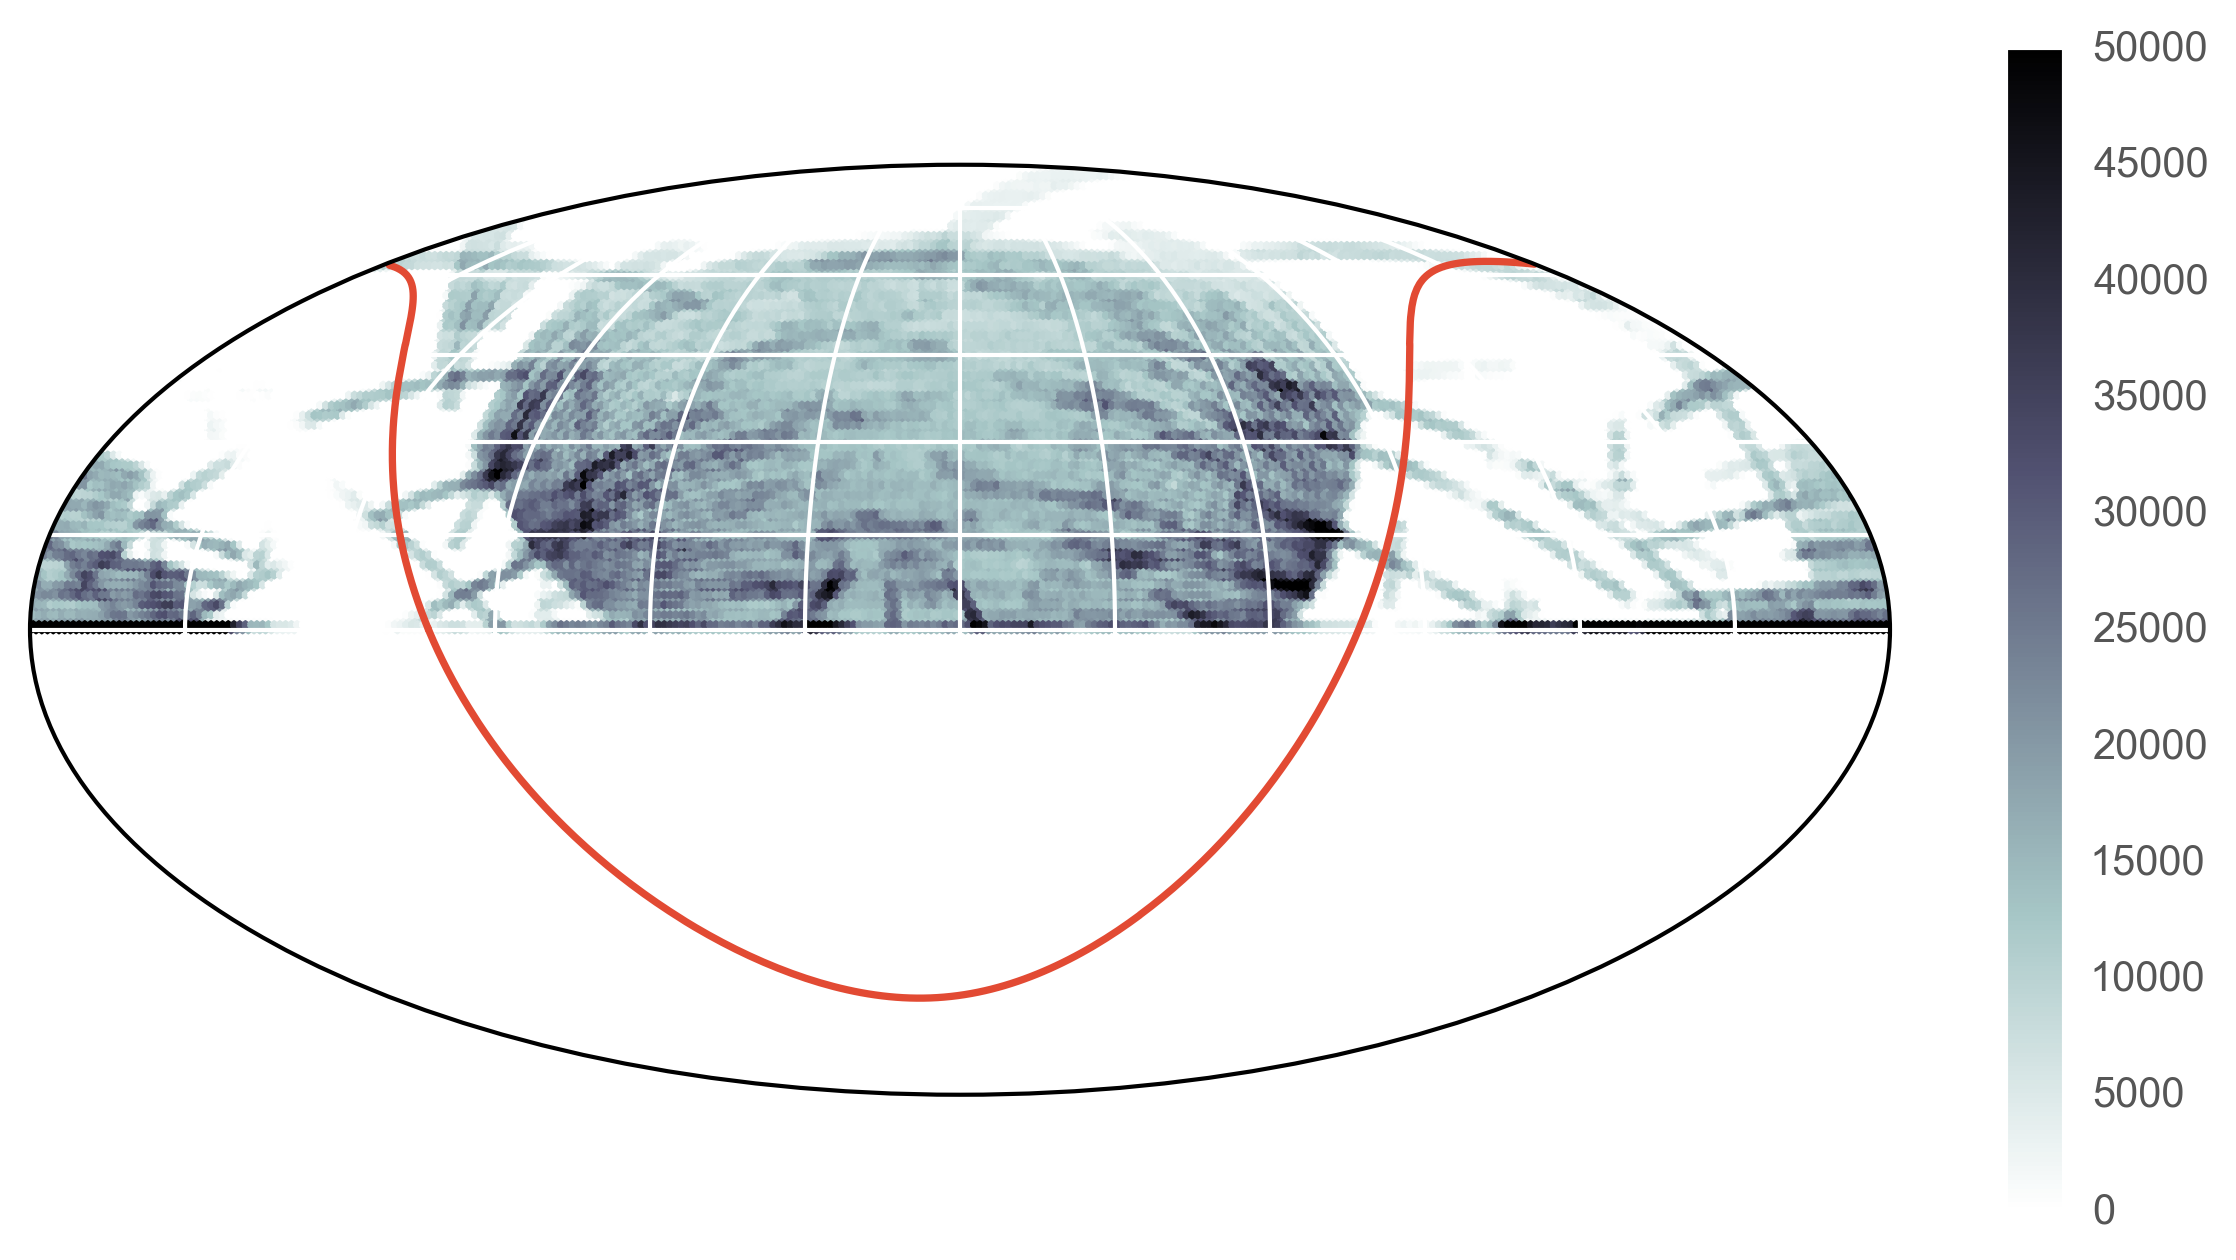
\includegraphics[width=0.75\textwidth]{figures/map_prediction_forest_galaxies}
		\caption{Distribution of galaxies.}
		\label{fig:random1}
	\end{subfigure}\\
	\begin{subfigure}{\textwidth}
		\centering
		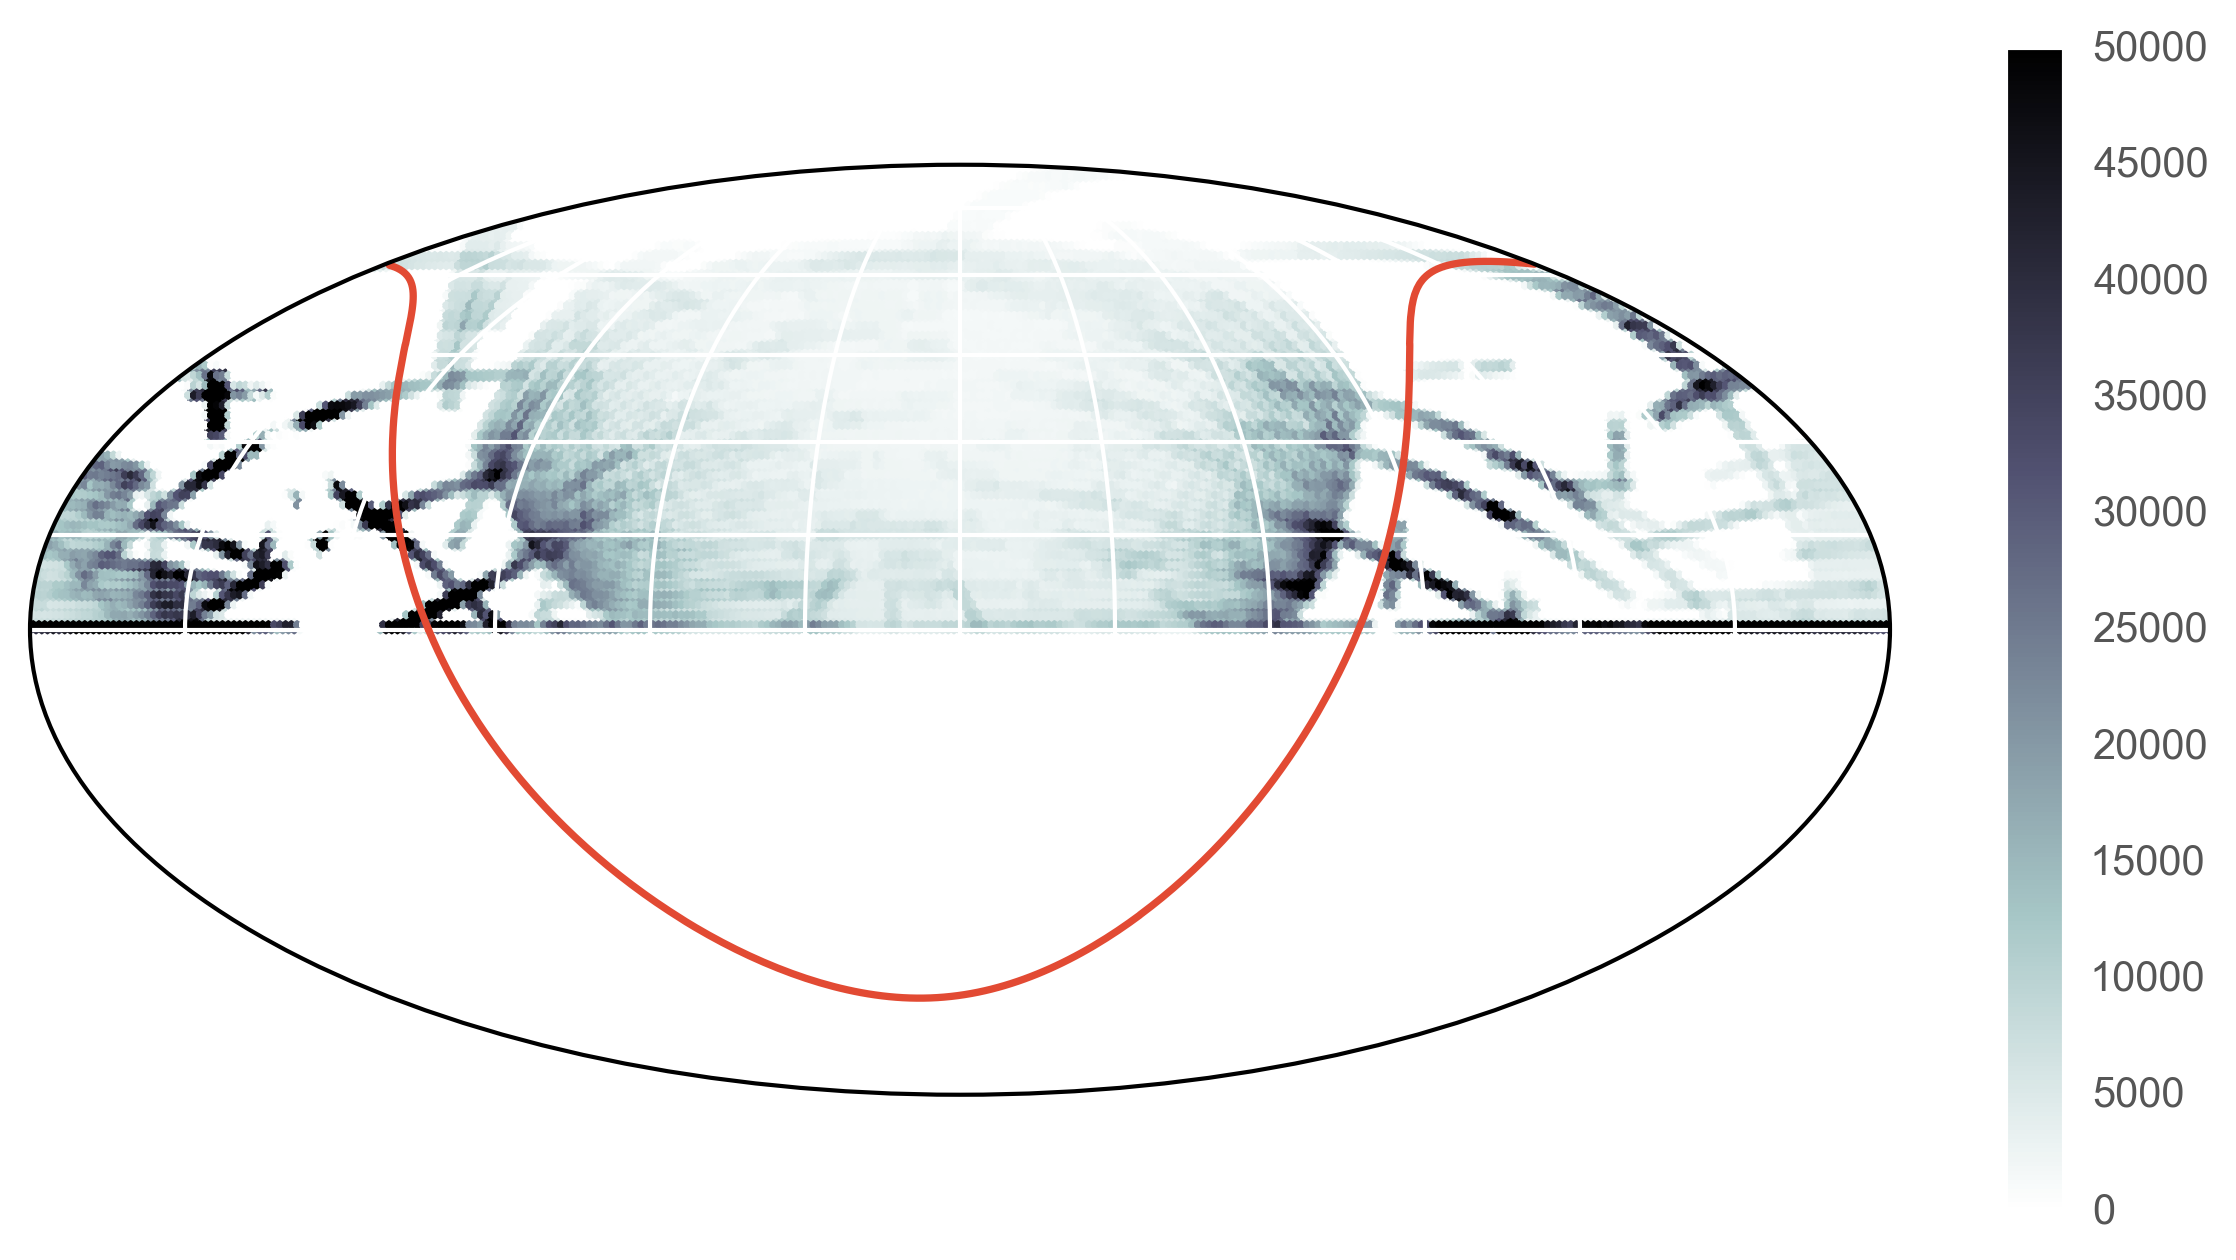
\includegraphics[width=0.75\linewidth]{figures/map_prediction_forest_stars}
		\caption{Distribution of stars.}
		\label{fig:random2}
	\end{subfigure}
	\begin{subfigure}{\textwidth}
		\centering
		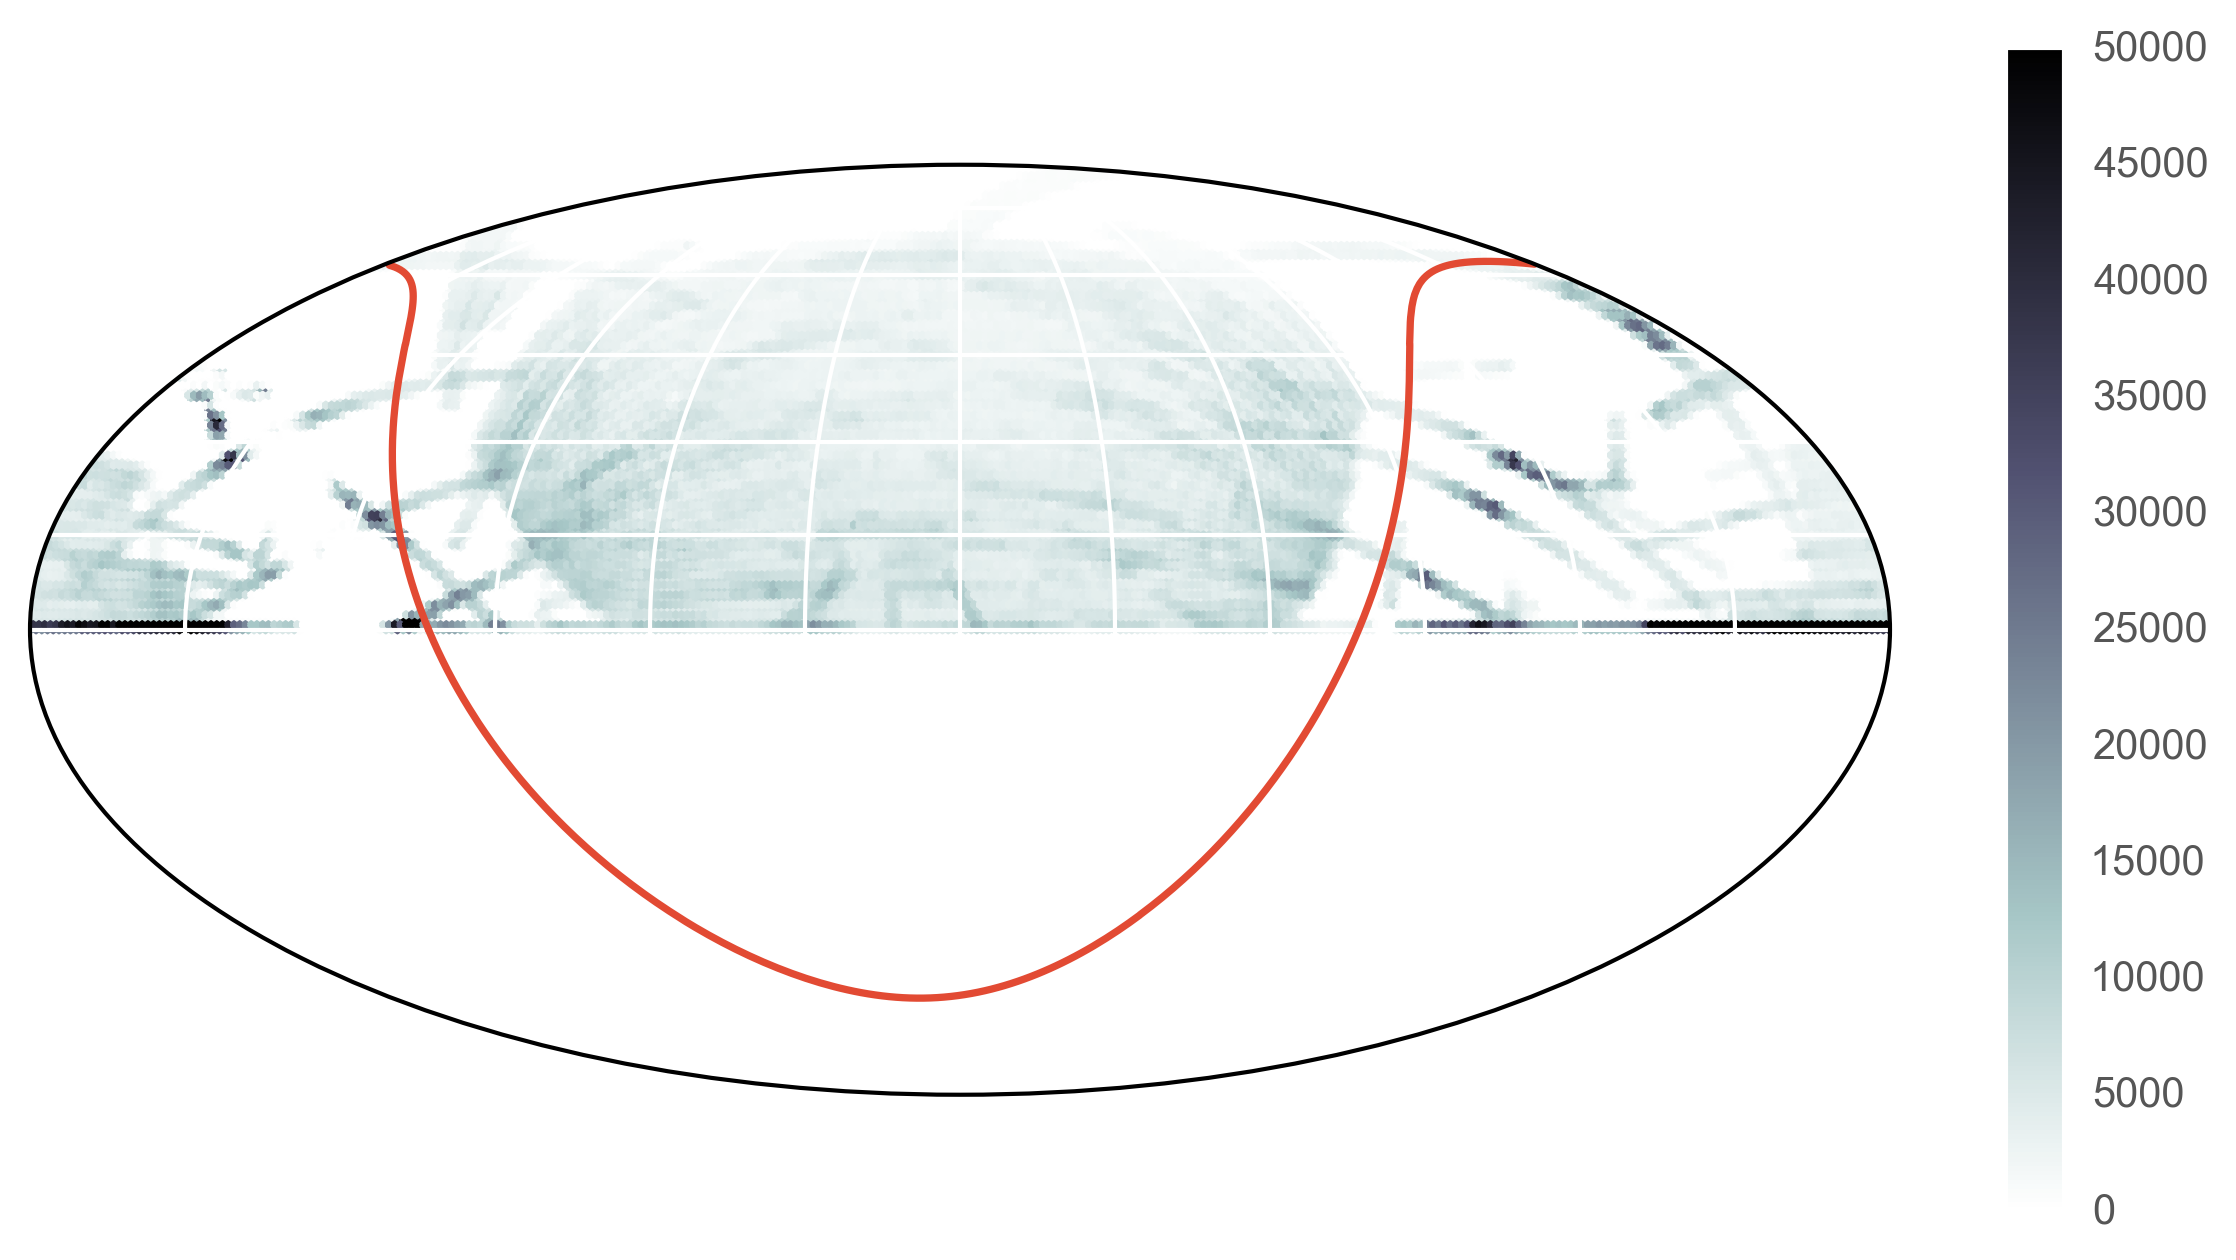
\includegraphics[width=0.75\linewidth]{figures/map_prediction_forest_quasars}
		\caption{Distribution of quasars.}
		\label{fig:random3}
	\end{subfigure}
	\caption{Map of predicted labels using random forest.}
	\label{fig:random}
\end{figure}


%%% Local Variables: 
%%% mode: latex
%%% TeX-master: "thesis"
%%% End: 
